\chapter{Methodological Approach to Requirement Engineering}
\section{Context Definition}
\subsection{Using Diagrams}
\begin{wrapfigure}{r}{0.5\textwidth}
    \centering
    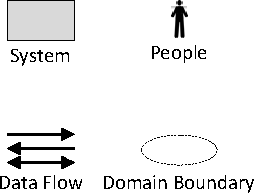
\includegraphics[scale=1]{img/SCDSymbols.pdf}
    \caption[Symbols of System Context Diagrams]{Symbols of System Context Diagrams \parencites[77]{Lauesen.2008}}
    \label{fig:scdSym}
\end{wrapfigure}
The system context diagram consists of four components: system, people, data flow, and domain boundaries \parencites[cf.][76-77]{Lauesen.2008}. Each one has its own representation, displayed in \Cref{fig:scdSym}. System context diagrams are used to identify required interfaces \parencites[cf.][75]{Lauesen.2008}, as well as to define the system boundary \parencites[cf.][75]{Ebert.2014}. It is an important overview of requirement sources, reflecting all interacting systems and persons. The direction of the arrow can show the direction of the data flow, or more commonly display the direction of intend \parencite[cf.][77]{Lauesen.2008}. In this paper the direction of an arrow will display the direction of intend.
\subsection{Using Personas}
Marketing communication applications have the quirk of having no direct impact of the targeted users on the product. They cannot directly be interviewed for goals and requirements. Additionally the group of targeted users is normaly to large to wrap your head around them. That is the reason for using personas. Human brains are caring more bout individuals, than large groups \parencite[cf.][]{Platt.2016}. Reasoning, archetypal individual people \parencite[cf.][81-82]{Cooper.2007}, which embody specific characteristics of groups \parencite[cf.][]{Platt.2016}. Identifying, analyzing, and prioritizing personas is a multistage procedure, which is always based on a type on research \parencite[cf.][39]{Robier.2016}. Research methods for this kind do not claim to scientifically acurate, but must not be based solely upon stereotypes and arbitrary decisions \parencite[cf.][82-83]{Cooper.2007}. 
\paragraph{} For identification of relevant stakeholders \textcite[38]{Robier.2016} suggest the usage of a stakeholder map (cf. \Cref{fig:stakeMap}). People of the left hand side of the vertical axis are the users of the program, divided into heavy users (far left) and fist time users (narrow to the axis) \parencite[cf.][38]{Robier.2016}. This approach aims not at the identification of each individual stakeholder, but at the identification of stakeholder groups to be represented by a persona \parencite[cf.][82]{Cooper.2007}, explicitly  including non-users \parencite[cf.][84]{Cooper.2007}.
\begin{figure}[H]
\centering
    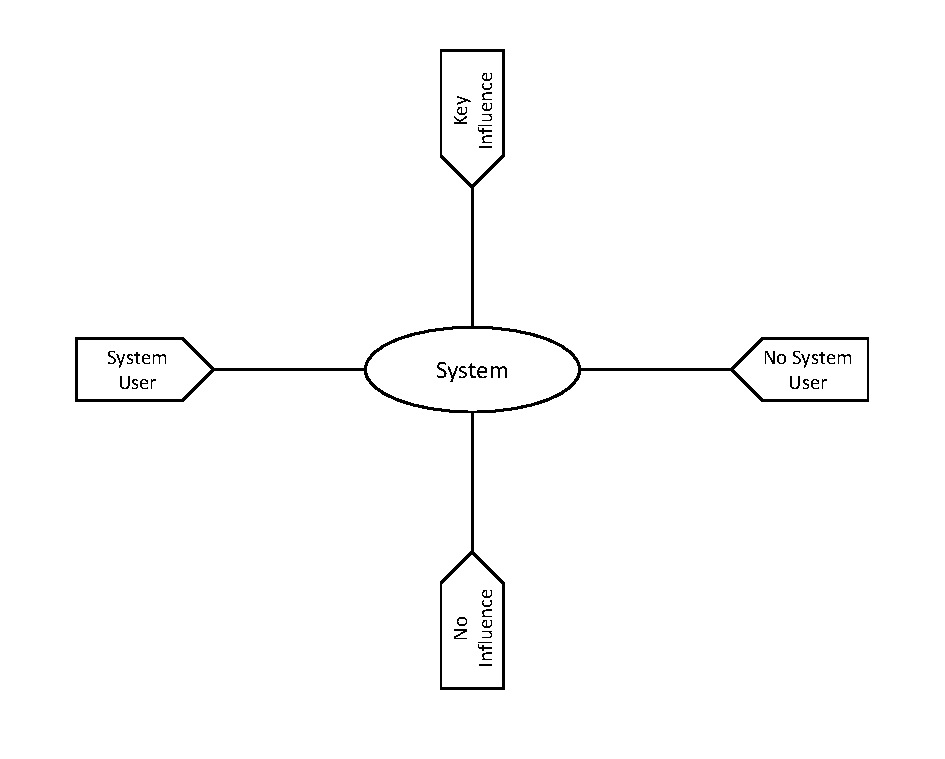
\includegraphics[scale=0.7]{img/stakeholderMap.pdf}
    \caption[Stakeholder Map]{Stakeholder Map (own illustration based on \cite[38]{Robier.2016})}
    \label{fig:stakeMap}
\end{figure}
Analysis of the personas identified, includes the specification of a personas traits. Since personas are represented as individual people \parencite[cf.][81]{Cooper.2007}, it has all attributes a natural person has, including a name, gender, age, family, education, and most importantly: a motivation \parencites[cf.][]{Platt.2016}[cf.][83-84]{Cooper.2007}. All traits of a persona must be contributing to a bigger picture, and thereby must be intentionally be set to suggest intended characteristics \parencite[cf.]{Platt.2016}. 
\paragraph{} As an example: Our persona Kevin Smith (25, male) works at a international bank as foreign trade manager after his studies in financial management at Harvard Business School and needs a way to plan his meetings in accordance to required travel times. In his free time he has a private single engine plane. If you ask yourself whether Kevin needs his schedule in a standardized time zone, such as UTC, the answer will definitely be yes, because he is on the one hand used to using UTC at work and in his hobby. Martha Jones (55, female) works at a local retailer since her diploma from community college, now being store manager, requiring a tool to plan and distribute shifts of her employees. She on the other hand will have more use for local time. Both may be personas for a calendar service focused on business customers. 
\paragraph{} All traits of Kevin and Martha will have implications on the conception and development of the hypothetical calendar service. Beside the very different functionality requests of transport service provider integration, respectively shift planning and public calendar provisioning, the age may have implications on the devices used, as well as the education implies different kinds of prior knowledge. 
\paragraph{} The prioritization of personas heavily depends on the specific product. It may be done by expected revenue (e.g. for sold services), least specialization (e.g. for training software) or any other reasonable technique for prioritization.
\begin{figure}[H]
    \centering
    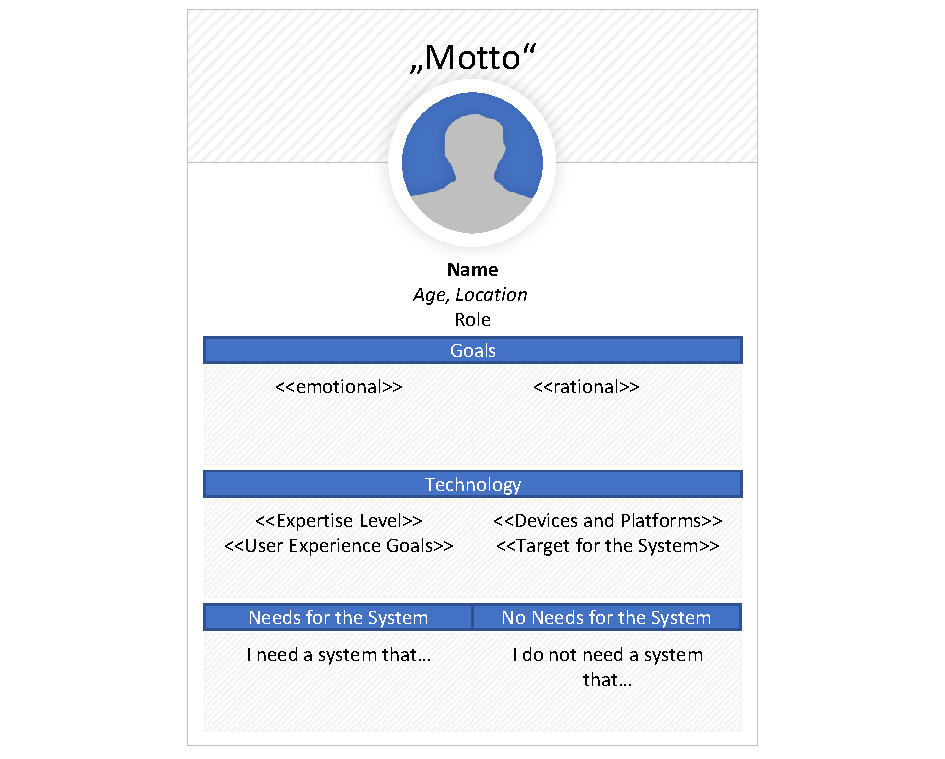
\includegraphics[scale=1]{img/PersonaTemplate.pdf}
    \caption[Template for Personas]{The template used for personas in this paper (own illustration)}
    \label{fig:persTemp}
\end{figure}
\paragraph{} The resulting personas are usually documented in a resume containing all relevant information \parencites[cf.][40]{Robier.2016}[cf.][]{Platt.2016}. This paper will use the template shown in \Cref{fig:persTemp}. It includes a picture of the persona, his or her personal information, his or her goals, needs, and for users his or her technological parameters.


\subsection{Sourcing Requirements from the Context}
Structuring in Facets
\clearpage
\subsection{Documentation}
\subsubsection{Natural Language Documentation of Goals}
Satzschablone
\begin{figure}[H]
    \centering
    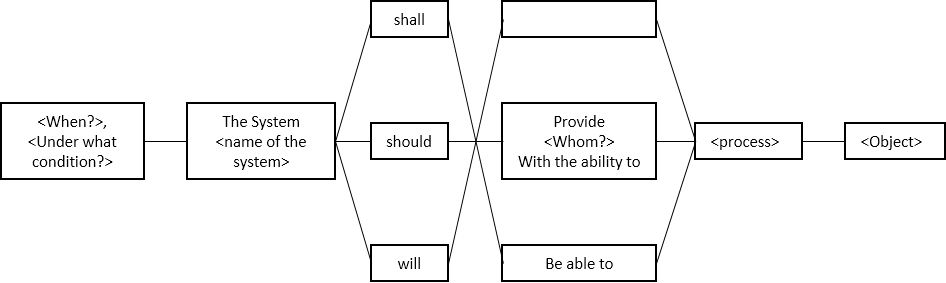
\includegraphics[width=\textwidth]{img/SentenceStructure.png}
    \caption{Requirement Documentation Sentence Structure (own illustration based on \cite[246]{Pohl.2007})}
    \label{fig:sentencestructure}
\end{figure}
\clearpage
\subsubsection{Diagram Notation for Scenarios}
For the documentation of scenarios, two types of diagram are recommended by \textcite[299]{Pohl.2007}. On the one hand, the use case diagram, which displays the goals of actors when interacting with the system, and on the other hand, sequence diagrams, which display the chronological set of interactions included in one use case.
\paragraph{} As mentioned above, use case diagrams consist actors, use cases and the system. It display in what kind the actors are directly or indirectly linked to the use cases. Actors can be generalized aggregations of other actors. As an example: business traveler and tourists are both visitors of hotels. They have different goals when visiting the hotel, but share some as well. The use case diagram will display the individual goals with the distinct actors, but generalize them to the visitor actor, which connects to the common goals. This example can be seen in \Cref{fig:ucEx}. As seen in \Cref{fig:ucEx}, the goals do not have to be connected directly to the actor.
\begin{figure}[H]
    \centering
    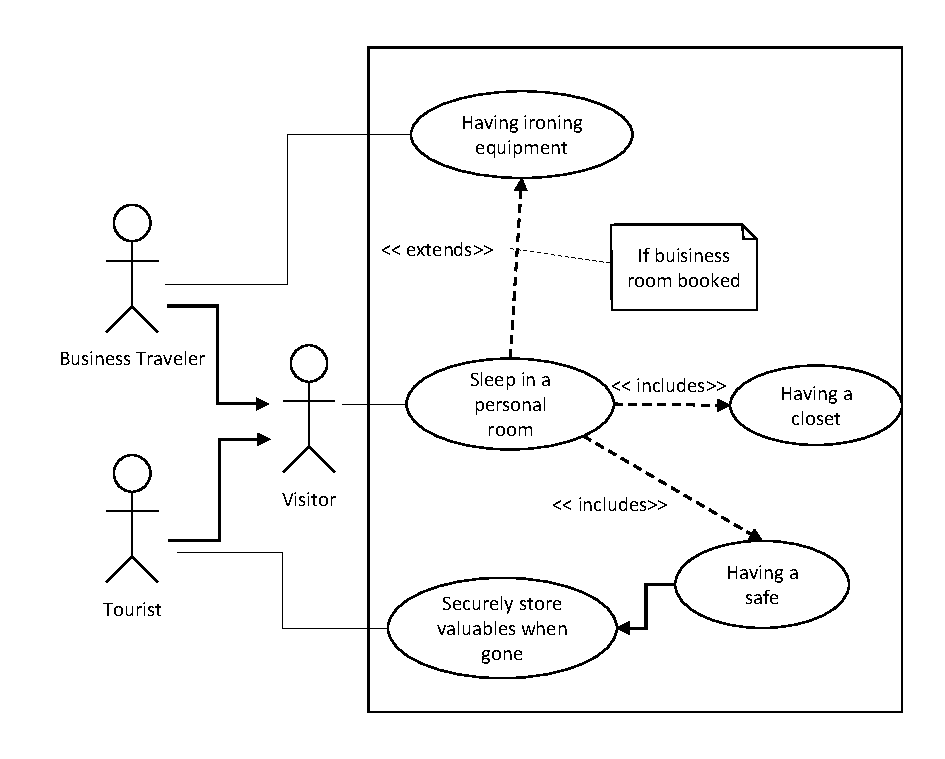
\includegraphics[scale=1]{img/ucEx.pdf}
    \caption[Example Use Case Diagram]{Use Case Diagram showing the Notation (own illustration)}
    \label{fig:ucEx}
\end{figure}
Aktivitätsdiagramm
\clearpage
\subsubsection{Diagram Notation for Solution Oriented Requirements}
Entity Relationship Model
Funktionsmodelle
Verhaltensmodelle
\clearpage
\subsection{Validating Conformity}
Scope Out
\clearpage
\chapter{Methodological Approach to User Interface Design}
\section{Outlining with Wire Frames}
\clearpage
\section{Prototyping with Mock-ups}
